\taskpic{ Через два неподвижных блока, находящихся на одной высоте,
  перекинута лёгкая нить, к концам которой прикреплены два груза
  одинаковой массы. Нить начинают медленно оттягивать вниз за точку,
  находящуюся посередине между блоками. График зависимости силы $F$,
  прикладываемой к нити, от смещения $x$ этой точки приведён на
  рисунке. Найдите массу $m$ каждого груза. Трения нет.  }
{
  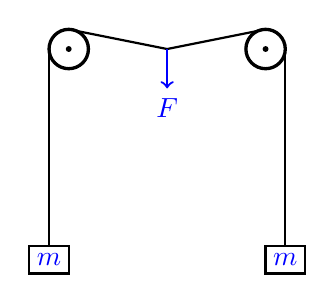
\begin{tikzpicture}
    \draw[very thick] (0.75,3) circle (0.25);
    \draw[very thick] (3.25,3) circle (0.25);
    \draw[thick] (0.5,0.5) -- (0.5,3);
    \draw[thick] (3.5,0.5) -- (3.5,3);
    \draw[thick] (0.8,3.24) -- (2,3) -- (3.2,3.24);
    \draw[thick,blue,->] (2,3) -- (2,2.5) node[below] {$F$};
    \draw[thick] (0.25,0.5) rectangle (0.75,0.15) node[midway,blue] {$m$};
    \draw[thick] (3.25,0.5) rectangle (3.75,0.15) node[midway,blue]
    {$m$};
    \draw[fill=black] (0.75,3) circle (0.03);
    \draw[fill=black] (3.25,3) circle (0.03);
  \end{tikzpicture}
}

\begin{center}
  \begin{tikzpicture}
    \begin{axis}[grid=major,smooth,xmin=0,ymin=0,xmax=5,ymax=10,y=0.3cm,xlabel={$x$, м}, ylabel={ $F$,
      Н}]
      \addplot[very thick,red,mark=none] { -10*exp(-x) + 10 };
    \end{axis}
  \end{tikzpicture}
\end{center}
% Московские физические олимпиады, 2000, 1.173
